\part{Configuration Guide}
{
\setlength{\parskip}{0em}
\DoPToC
}

% ----------------------------------------------------------------

\chapter{FC7 Configuration}

\section{Configuration Parameters}

The FC7 needs to switch automatically among different modes, according to a predetermined sequence.  This sequence will be configurable via IPbus with a dedicated slave.

The switching among modes primarily refers to changing trigger modes, such as muon fills, laser runs, pedestal runs, and asynchronous crate readouts.  For the Rider, this is accomplished by changing the TTC Channel B command with or prior to the TTC Channel A trigger.  For the laser system, this is accomplished by outputting a trigger signal after a set delay for only laser runs.

A diagram of such a trigger sequence scheme is shown in Figure~\ref{trig-seq}.  Each step of the sequence is defined by a trigger index, trigger type, and pre-trigger gap.  These three parameters are defined in Table~\ref{fc7-param}.  Note that each sequence is synchronous to the accelerator trigger, and, at the end of the sequence, the FC7 will wait for the next accelerator trigger.

\begin{figure}[b]
\centering
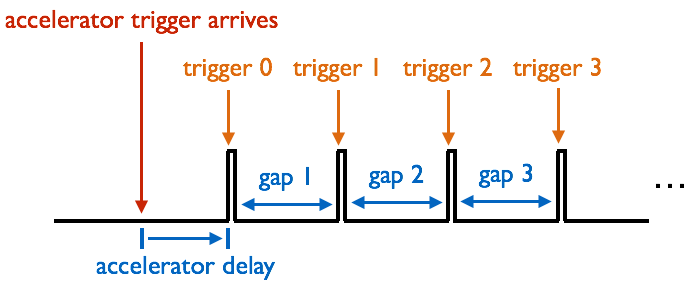
\includegraphics[width=0.85\textwidth]{images/trigger_sequence.png}
\caption{FC7 trigger sequence scheme.}
\label{trig-seq}
\end{figure}

\newpage

It would also be possible to define multiple trigger sequences.  This would require similar parameters to determine the order and rate that each sequence is executed.  A multi-sequence behavior could be advantageous for certain triggers, such as the asynchronous crate readout, that need to be issued but not very often.

In addition, multiple trigger sequences will be integral to running the \gm2 experiment, simply because of the bunch structure within each super-cycle.  In each super-cycle, there will be two groups of eight muon bunches that are separated by 10~ms.  There is a 197~ms gap after the first bunch group and a 1063~ms gap after the second bunch group.  We will definitely want to execute a difference set of sequences during the three different gaps (10~ms, 197~ms, 1063~ms).

{
\renewcommand{\arraystretch}{1.25}
\begin{table}[t]
\centering
\begin{tabular}{| l | l |}
\hline
Parameter                	& Description \\ \hline \hline
Trigger Index  		& Index of trigger in sequence, starting at zero. \\
Trigger Type  		& Type of trigger (muon, laser, pedestal, asynchronous readout). \\ 
Pre-Trigger Gap   	& Number of 40-MHz TTC clock cycles to wait before issuing trigger. \\
\hline
\end{tabular}
\caption{FC7 triggering parameters that are configurable via IPbus.}
\label{fc7-param}
\end{table}
}

\section{Configuration Logic}

The implementation of trigger sequences should be straightforward.  A dedicated IPbus slave should be created that holds a memory of 32 32-bit registers.  These registers will hold the trigger type and pre-trigger gap for each index of the sequence.  The total number of indices in the sequence will also need to be specified in one of the registers.

These IPbus registers will then be used in a finite state machine.  An idea of what this state machine might look like is pictured in Figure~\ref{seq-sm}.  The state machine will be initialized to the \verb|IDLE| state, where it waits for the (already delayed) front panel trigger.  When it sees the trigger, it will transition to the \verb|SEND_TRIGGER| state, which sets the TTC Channel A to issue a trigger.

If that was the last trigger in the sequence, the state machine transitions back to \verb|IDLE|.  If there is another index in the sequence, it will instead transition to the \verb|SEND_COMMAND| state.  It stays here until the proper TTC Channel B command is issued, setting the next trigger type, and, when done, moves to \verb|WAIT|.  The state machine will then pause until the pre-trigger gap period has expired.  At that point, it will move back to the \verb|SEND_TRIGGER| state and repeat the logical process.

\subsection{Timing Specifications}

Recall that the TTC data is encoded in two alternating channels.  The Channel A encodes the 1-bit trigger signal, while the Channel B encodes the 8-bit broadcast command with an 8-bit overhead.  In each 40-MHz clock cycle, one bit of each channel is sent.  This means that 16 clock cycles are required to send the command to switch fill types and, therefore, the minimum delay between different trigger types is 425~ns, after accounting for the one clock cycle enforced by the \verb|WAIT|.

In the FC7 firmware, caution must be taken to ensure proper synchronization of signals.  This is especially important the signals cross clock domains, which is the case for all signals going from the 125-MHz IPbus clock domain and to the 40-MHz trigger logic clock domain.

\begin{figure}[t]
\centering
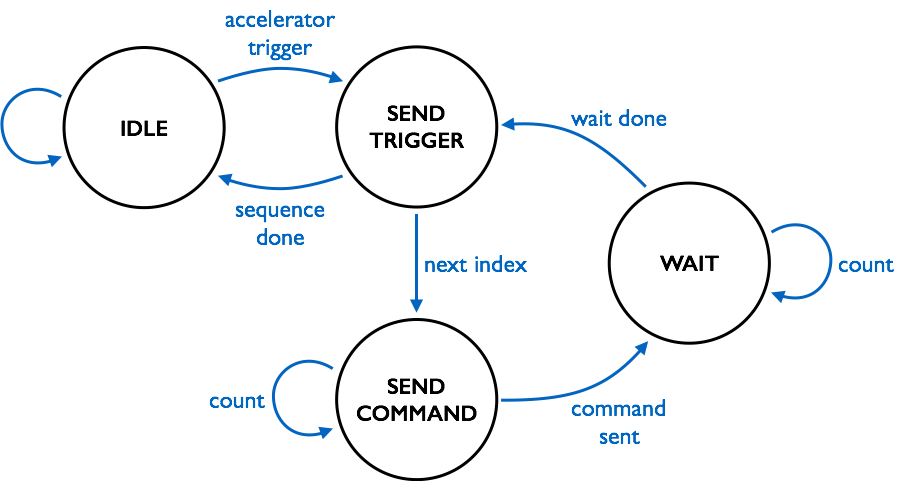
\includegraphics[width=0.90\textwidth]{images/seq_sm2.png}
\caption{State machine diagram for implementing FC7 trigger sequence.}
\label{seq-sm}
\end{figure}

\subsection{Broadcast Commands}

The Channel B of the TTC protocol encodes an 8-bit broadcast command.  In the calorimeter system, the broadcast commands are used to switch trigger types (muon fill, laser, pedestal, asynchronous readout) on the waveform digitizers, i.e., Riders.  The valid broadcast commands that are recognized by the Riders are listed and described in Table~\ref{broadcast}.  Note that the \emph{Event-Count Reset} and \emph{Counter Reset} commands are also recognized by the AMC13.

{
\renewcommand{\arraystretch}{1.25}
\begin{table}[t]
\centering
\begin{tabular}{| l | l | l |}
\hline
Command 				& Broadcast [7:0]	& Meaning \\ \hline \hline
Event-Count Reset 			& \verb|xxxxxx1x| 	& Reset event counter \\
Counter Reset 				& \verb|001x1xxx| 	& Reset 44-bit counter used for timestamps \\ \hline
Async. Readout Trigger Type	& \verb|100x0xxx| 	& Switch to ``Async. Readout" trigger type \\
Muon Trigger Type 			& \verb|101x0xxx| 	& Switch to ``Muon Fill" trigger type \\
Laser Trigger Type 			& \verb|110x0xxx| 	& Switch to ``Laser" trigger type \\
Pedestal Trigger Type		& \verb|111x0xxx|	& Switch to ``Pedestal" trigger type \\ \hline
Start Async. Pulse Storage 	& \verb|100x1xxx| 	& Start accepting front panel triggers \\
Stop Async. Pulse Storage 	& \verb|101x1xxx| 	& Stop accepting front panel triggers \\
\hline
\end{tabular}
\caption{Valid broadcast commands recognized by the Riders.}
\label{broadcast}
\end{table}
}
